% JEFE 1 — Tesis completa: varios archivos y carpetas, biber, glosario, siglas, nomenclatura,
% dos índices alfabéticos, referencias cruzadas, tablas largas, gráficas desde un .csv e imágenes
% con espacios y tildes en el nombre. Todo junto, como una tesis real de Overleaf.
\documentclass[11pt,a4paper,oneside]{report}
\usepackage[T1]{fontenc}
\usepackage[spanish,es-noshorthands]{babel}
\usepackage{lmodern}
\usepackage[margin=2.5cm]{geometry}
\usepackage{csquotes}
\usepackage{amsmath,amssymb}
\usepackage{graphicx}
\usepackage{subcaption}
\usepackage{booktabs,longtable,multirow,threeparttable,array}
\usepackage[table]{xcolor}
\usepackage{siunitx}
\sisetup{output-decimal-marker={,}, group-separator={\,}}
\usepackage{pgfplots}
\pgfplotsset{compat=1.18}
\usepackage[american]{circuitikz}
\usepackage{listings}
\usepackage[backend=biber,style=authoryear,maxcitenames=2]{biblatex}
\addbibresource{referencias.bib}
\usepackage{imakeidx}
\makeindex[intoc]
\makeindex[name=autores,title={Índice de autores},intoc]
\usepackage[intoc,spanish]{nomencl}
\makenomenclature
\usepackage{hyperref}
\hypersetup{colorlinks, linkcolor=blue!50!black, citecolor=green!40!black, urlcolor=teal}
\usepackage[spanish,capitalise]{cleveref}
\usepackage[acronym,toc,nonumberlist]{glossaries}
\makeglossaries
\newacronym{rlc}{RLC}{resistencia, inductancia y capacitancia}
\newacronym{ca}{CA}{corriente alterna}
\newacronym{fft}{FFT}{transformada rápida de Fourier}
\newglossaryentry{fasor}{name={fasor}, description={número complejo que representa la amplitud y la fase de una señal sinusoidal}}
\newglossaryentry{impedancia}{name={impedancia}, description={oposición total de un circuito al paso de la \gls{ca}, en ohmios}}
\newglossaryentry{resonancia}{name={resonancia}, description={frecuencia a la que la reactancia inductiva y la capacitiva se anulan}}

\usepackage{todonotes}

\lstset{basicstyle=\ttfamily\small, columns=fullflexible, frame=single, breaklines=true,
  literate={á}{{\'a}}1 {é}{{\'e}}1 {í}{{\'i}}1 {ó}{{\'o}}1 {ú}{{\'u}}1 {ñ}{{\~n}}1 {Ñ}{{\~N}}1}

\title{Caracterización de un circuito RLC\\[4pt]\large Tesis de prueba para TeXsting}
\author{Pedro de la Cruz Castillo}
\date{\today}

\begin{document}
\maketitle
\pagenumbering{roman}
\tableofcontents
\listoffigures
\listoftables
\printglossary[type=\acronymtype, title={Siglas}]
\printglossary[title={Glosario}]
\printnomenclature
\cleardoublepage
\pagenumbering{arabic}

\chapter{Introducción}\label{cap:intro}
Un circuito \gls{rlc} es el ejemplo clásico de sistema de segundo orden~\parencite{alexander2013,nilsson2015}.
Su respuesta en \gls{ca} se estudia con \glspl{fasor} y con la \gls{impedancia}; el análisis en
frecuencia moderno usa la \gls{fft}~\parencite{cooley1965}. Como resume \textcite{ogata2010},
\enquote{todo sistema lineal se entiende mejor en el dominio de la frecuencia}.
\index{circuito RLC}\index{fasor}\index[autores]{Alexander, C.}\index[autores]{Cooley, J. W.}

La frecuencia de \gls{resonancia} es
\begin{equation}\label{eq:resonancia}
  \omega_0 = \frac{1}{\sqrt{LC}}, \qquad f_0 = \frac{1}{2\pi\sqrt{LC}},
\end{equation}
\nomenclature{$\omega_0$}{Frecuencia angular de resonancia \nomunit{\si{\radian\per\second}}}%
\nomenclature{$L$}{Inductancia \nomunit{\si{\henry}}}%
\nomenclature{$C$}{Capacitancia \nomunit{\si{\farad}}}%
\nomenclature{$R$}{Resistencia \nomunit{\si{\ohm}}}%
y el factor de calidad $Q = \frac{1}{R}\sqrt{L/C}$. En el \cref{cap:mediciones} se mide $f_0$ y en el
\cref{cap:resultados} se compara con la \cref{eq:resonancia}. Los datos crudos están en el
\cref{ap:codigo}.\index{resonancia|textbf}

\section{Objetivos}
\begin{enumerate}
  \item Medir la respuesta en frecuencia (ver \cref{tab:mediciones}).
  \item Verificar la \cref{eq:resonancia} con un error menor a \SI{5}{\percent}.\todo{¿5 \% es suficiente?}
  \item Comparar con la simulación de \textcite[cap.~14]{nilsson2015} y con la norma~\parencite{ieee1057}.
\end{enumerate}

\section{Antecedentes}
Trabajos previos~\parencite{tesisperez,datasheet} muestran que el modelo ideal falla por encima de
\SI{1}{\mega\hertz}.\index[autores]{Pérez, M.}\index{modelo ideal}

\chapter{Mediciones}\label{cap:mediciones}
El montaje de la \cref{fig:montaje} usa los valores $R=\SI{47}{\ohm}$, $L=\SI{10}{\milli\henry}$ y
$C=\SI{100}{\nano\farad}$.\index{montaje experimental}

\begin{figure}[htbp]
  \centering
  \begin{subfigure}[b]{0.48\textwidth}
    \centering
    \begin{circuitikz}[scale=0.85, transform shape]
      \draw (0,0) to[sV, l=$v_s(t)$] (0,3)
            to[R, l=$R$, -*] (3,3)
            to[L, l=$L$] (5,3)
            to[C, l=$C$, v^>=$v_C$] (5,0) -- (0,0);
    \end{circuitikz}
    \caption{Esquema.}\label{fig:esquema}
  \end{subfigure}\hfill
  \begin{subfigure}[b]{0.48\textwidth}
    \centering
    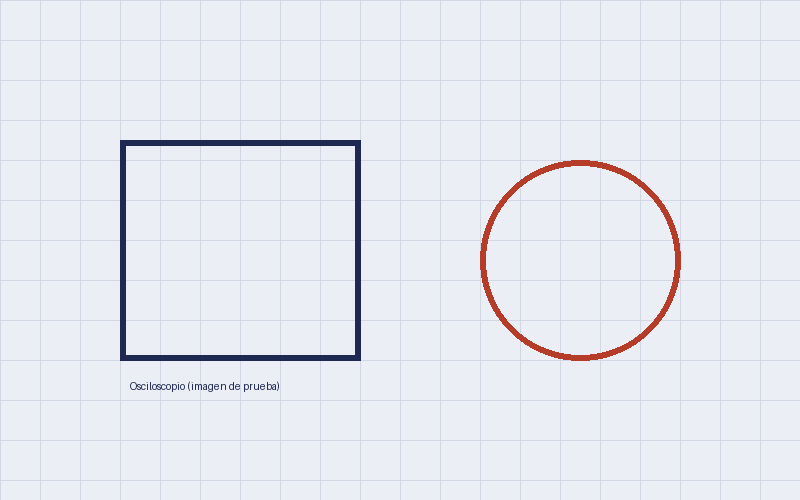
\includegraphics[width=\linewidth]{figuras/foto del laboratorio.png}
    \caption{Montaje real.}\label{fig:foto}
  \end{subfigure}
  \caption{Circuito \gls{rlc} serie usado en las mediciones.}\label{fig:montaje}
\end{figure}

\begin{figure}[htbp]
  \centering
  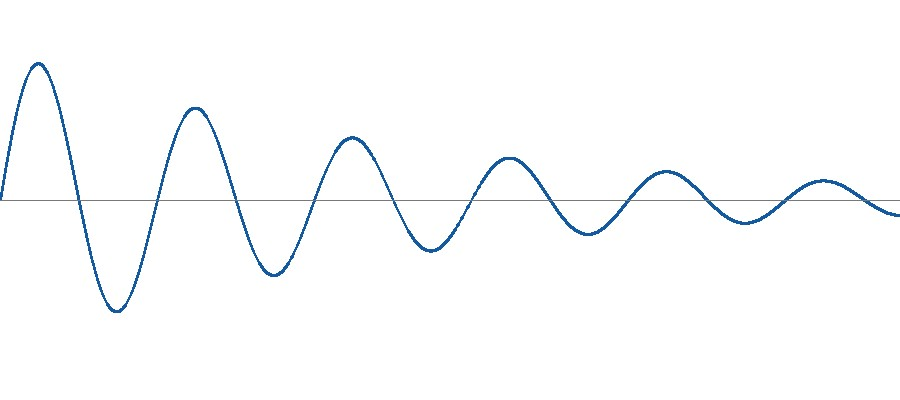
\includegraphics[width=0.8\textwidth]{figuras/señal medida.jpg}
  \caption{Señal medida en el osciloscopio (nombre de archivo con tilde y espacio).}\label{fig:senal}
\end{figure}

\section{Tabla de mediciones}
La \cref{tab:mediciones} es larga a propósito: cruza de página y repite su encabezado.

\begin{longtable}{
  S[table-format=6.0]
  S[table-format=2.3]
  S[table-format=2.3]
  S[table-format=+3.1]
  c}
  \caption{Respuesta en frecuencia medida.}\label{tab:mediciones}\\
  \toprule
  {$f$ (\si{\hertz})} & {$V_\text{in}$ (\si{\volt})} & {$V_C$ (\si{\volt})} & {$\varphi$ (\si{\degree})} & {Nota}\\
  \midrule
  \endfirsthead
  \multicolumn{5}{l}{\small\itshape (continuación de la \cref{tab:mediciones})}\\
  \toprule
  {$f$ (\si{\hertz})} & {$V_\text{in}$ (\si{\volt})} & {$V_C$ (\si{\volt})} & {$\varphi$ (\si{\degree})} & {Nota}\\
  \midrule
  \endhead
  \midrule\multicolumn{5}{r}{\small\itshape sigue en la página siguiente}\\
  \endfoot
  \bottomrule
  \endlastfoot
  100 & 2.000 & 2.001 & -0.2 & \\
  112 & 2.000 & 2.001 & -0.2 & \\
  125 & 2.000 & 2.001 & -0.2 & \\
  140 & 2.000 & 2.002 & -0.2 & \\
  156 & 2.000 & 2.002 & -0.3 & \\
  174 & 2.000 & 2.002 & -0.3 & \\
  194 & 2.000 & 2.003 & -0.3 & \\
  217 & 2.000 & 2.004 & -0.4 & \\
  243 & 2.000 & 2.005 & -0.4 & \\
  272 & 2.000 & 2.006 & -0.5 & \\
  304 & 2.000 & 2.007 & -0.5 & \\
  340 & 2.000 & 2.009 & -0.6 & \\
  380 & 2.000 & 2.011 & -0.6 & \\
  425 & 2.000 & 2.014 & -0.7 & \\
  476 & 2.000 & 2.018 & -0.8 & \\
  533 & 2.000 & 2.022 & -0.9 & \\
  596 & 2.000 & 2.028 & -1.0 & \\
  667 & 2.000 & 2.035 & -1.1 & \\
  747 & 2.000 & 2.045 & -1.3 & \\
  836 & 2.000 & 2.056 & -1.5 & \\
  936 & 2.000 & 2.071 & -1.6 & \\
  1048 & 2.000 & 2.090 & -1.9 & \\
  1173 & 2.000 & 2.113 & -2.1 & \\
  1313 & 2.000 & 2.144 & -2.4 & \\
  1470 & 2.000 & 2.184 & -2.7 & \\
  1646 & 2.000 & 2.236 & -3.1 & \\
  1843 & 2.000 & 2.305 & -3.6 & \\
  2064 & 2.000 & 2.398 & -4.2 & \\
  2311 & 2.000 & 2.525 & -4.9 & \\
  2588 & 2.000 & 2.704 & -5.9 & \\
  2898 & 2.000 & 2.968 & -7.3 & \\
  3245 & 2.000 & 3.378 & -9.3 & \\
  3634 & 2.000 & 4.077 & -12.6 & \\
  4070 & 2.000 & 5.460 & -19.2 & \\
  4170 & 2.000 & 5.938 & -21.4 & \\
  4270 & 2.000 & 6.509 & -24.2 & \\
  4370 & 2.000 & 7.198 & -27.7 & \\
  4470 & 2.000 & 8.031 & -32.0 & \\
  4570 & 2.000 & 9.034 & -37.6 & \\
  4670 & 2.000 & 10.213 & -44.8 & \\
  4770 & 2.000 & 11.510 & -54.2 & \\
  4870 & 2.000 & 12.715 & -66.1 & \\
  4970 & 2.000 & 13.436 & -80.4 & \\
  5070 & 2.000 & 13.293 & -95.6 & \\
  5170 & 2.000 & 12.319 & -109.9 & \\
  5270 & 2.000 & 10.924 & -121.8 & \\
  5370 & 2.000 & 9.501 & -131.1 & \\
  5470 & 2.000 & 8.238 & -138.3 & \\
  5570 & 2.000 & 7.180 & -143.8 & \\
  5670 & 2.000 & 6.309 & -148.1 & \\
  5770 & 2.000 & 5.593 & -151.5 & \\
  5870 & 2.000 & 5.002 & -154.3 & \\
  5970 & 2.000 & 4.509 & -156.6 & \\
  6070 & 2.000 & 4.093 & -158.5 & \\
  6798 & 2.000 & 2.357 & -166.3 & \\
  7613 & 2.000 & 1.530 & -170.1 & \\
  8526 & 2.000 & 1.060 & -172.3 & \\
  9549 & 2.000 & 0.765 & -173.8 & \\
  10694 & 2.000 & 0.567 & -174.9 & \\
  11977 & 2.000 & 0.428 & -175.7 & \\
  13414 & 2.000 & 0.327 & -176.3 & \\
  15023 & 2.000 & 0.252 & -176.8 & \\
  16825 & 2.000 & 0.196 & -177.2 & \\
  18844 & 2.000 & 0.153 & -177.6 & \\
  21105 & 2.000 & 0.121 & -177.8 & \\
  23637 & 2.000 & 0.095 & -178.1 & \\
  26473 & 2.000 & 0.075 & -178.3 & \\
  29649 & 2.000 & 0.059 & -178.5 & \\
  33206 & 2.000 & 0.047 & -178.7 & \\
  37190 & 2.000 & 0.037 & -178.8 & \\
  41652 & 2.000 & 0.030 & -179.0 & \\
  46650 & 2.000 & 0.024 & -179.1 & \\
  52248 & 2.000 & 0.019 & -179.2 & \\
  58517 & 2.000 & 0.015 & -179.3 & \\
  65539 & 2.000 & 0.012 & -179.3 & \\
  73403 & 2.000 & 0.009 & -179.4 & \\
  82211 & 2.000 & 0.008 & -179.5 & \\
  92076 & 2.000 & 0.006 & -179.5 & \\
  103125 & 2.000 & 0.005 & -179.6 & \\
  115500 & 2.000 & 0.004 & -179.6 & \\
  129360 & 2.000 & 0.003 & -179.7 & \\
  144883 & 2.000 & 0.002 & -179.7 & \\
  162268 & 2.000 & 0.002 & -179.7 & \\
  181740 & 2.000 & 0.002 & -179.8 & \\
\end{longtable}

\section{Resumen con notas al pie en la tabla}
\begin{table}[htbp]
  \centering
  \begin{threeparttable}
    \caption{Comparación teórica y medida.}\label{tab:resumen}
    \rowcolors{2}{gray!10}{white}
    \begin{tabular}{l S[table-format=4.1] S[table-format=4.1] S[table-format=1.2]}
      \toprule
      Magnitud & {Teórico} & {Medido} & {Error (\si{\percent})}\\
      \midrule
      $f_0$ (\si{\hertz})\tnote{a} & 5032.9 & 5010.0 & 0.45\\
      $Q$\tnote{b} & 6.7 & 6.4 & 4.48\\
      \multirow{2}{*}{Ancho de banda (\si{\hertz})} & 751.0 & 782.0 & 4.13\\
       & 751.0 & 779.5 & 3.79\\
      \bottomrule
    \end{tabular}
    \begin{tablenotes}\footnotesize
      \item[a] Con la \cref{eq:resonancia}.
      \item[b] $Q=f_0/\Delta f$.
    \end{tablenotes}
  \end{threeparttable}
\end{table}

\chapter{Resultados}\label{cap:resultados}
La \cref{fig:bode} se dibuja directamente desde \texttt{datos/mediciones.csv}.\index{diagrama de Bode}

\begin{figure}[htbp]
  \centering
  \begin{tikzpicture}
    \begin{semilogxaxis}[width=0.9\textwidth, height=6cm, grid=both,
        xlabel={Frecuencia (\si{\hertz})}, ylabel={$|H|$ (\si{\decibel})},
        legend pos=south west]
      \addplot[blue, thick] table[x=f, y=db, col sep=semicolon] {datos/mediciones.csv};
      \addlegendentry{medido}
      \addplot[red, dashed, domain=100:200000, samples=200]
        {20*log10(1/sqrt((1-(2*pi*x)^2*1e-9)^2 + (2*pi*x*47*1e-7)^2))};
      \addlegendentry{teórico}
      \draw[gray, dotted] (axis cs:5033,-60) -- (axis cs:5033,20) node[above, black, font=\small] {$f_0$};
    \end{semilogxaxis}
  \end{tikzpicture}
  \caption{Diagrama de Bode: medición (archivo \texttt{.csv}) frente a teoría.}\label{fig:bode}
\end{figure}

\section{Discusión}
El error de $f_0$ es \SI{0.45}{\percent} (\cref{tab:resumen}), dentro del objetivo. La forma de la
curva de la \cref{fig:senal} coincide con la respuesta subamortiguada de \textcite{alexander2013}.
\index{error de medición}\index[autores]{Ogata, K.}


\appendix
\chapter{Código del análisis}\label{ap:codigo}
El cálculo se hizo con este programa (con tildes y eñes en los comentarios):
\begin{lstlisting}[language=Python, caption={Cálculo de la respuesta en frecuencia}]
import numpy as np
R, L, C = 47, 10e-3, 100e-9   # valores del montaje (año 2026, señal de prueba)
f = np.logspace(2, 5.3, 400)
w = 2*np.pi*f
H = 1/(1 - w**2*L*C + 1j*w*R*C)
print("Resonancia:", 1/(2*np.pi*np.sqrt(L*C)), "Hz")
\end{lstlisting}

Y una salida literal con caracteres especiales:
\begin{verbatim}
$ ./medir --rango=100:200000 --paso=1.12 > datos/mediciones.csv   # % & _ { } ~ ^ \
\end{verbatim}


\printbibliography[heading=bibintoc, title={Referencias}]
\printindex
\printindex[autores]
\end{document}
